\documentclass[5pt]{article}
    \title{\textbf{1. MĚŘENÍ ANALOGOVÝM OSCILOSKOPEM}}
    \author{Tomáš Kysela}
    \date{16/2/2022}
    
    \addtolength{\topmargin}{-3cm}
    \addtolength{\textheight}{3cm}
    
\usepackage[czech]{babel}
\usepackage{graphicx}
\usepackage{circuitikz}
\usepackage{amsmath}
\usepackage{subcaption}
\begin{document}

\maketitle
\thispagestyle{empty}

\section{Úkol měření}
\begin{enumerate}
\item Na základě popisu uvedeného v Teoretickém úvodu se  seznamte  s funkcí analogového laboratorního osciloskopu.
\item S použitím jednokanálového režimu zobrazte na analogovém osciloskopu průběh napětí v bodě K1 popř. K2  astabilního  klopného  obvodu.  Zesílení,  vertikální  posuv (skupina  ovládacích  prvků „vertical“)  a rychlost běhu ČZ (skupina ovládacích prvků „horizontal“) nastavte tak, aby zobrazení bylo optimální. Nastavte režim spouštění „AUTO“ signálem z použitého kanálu, sledujte vliv změny nastavení  spouštěcí  úrovně,  popř.  spouštění  náběžnou  a  sestupnou  hranou  na  zobrazený  signál (skupina ovládacích prvků „trigger“). Totéž vyzkoušejte v režimu „NORM“.
\item U zobrazeného průběhu určete frekvenci, $U_{min}$,  $U_{max}$, střední hodnotu (stejnosměrnou složku), trvání vzestupné  a  sestupné  hrany.  Pozor,  hodnoty  pro  rychlost  běhu  ČZ  a  citlivosti  platí  pouze  jsou-li plynulá nastavení v poloze „kalibrováno“ (cal).
\item S použitím dvoukanálového režimu zobrazte na analogovém osciloskopu průběhy  napětí v bodě K1 popř. K2 a B1 popř. B2 astabilního klopného obvodu.
\item S využitím nf generátoru a napětí 6 V o kmitočtu 50 Hz (z rozvaděče) ověřte funkci režimu X-Y osciloskopu (Lissajoussovy obrazce).
\item Body  2  a  3  zopakujte  s použitím číslicového osciloskopu (popis ovládacích prvků je podobný). Pro základní nastavení ovládacích prvků použijte tlačítko „Auto Scale“. Povšimněte si rozdílů v zobrazení (bod  „trig“  je  při  základním  nastavení  uprostřed  a  je  tedy  zobrazen  i  průběh  signálu  před  jeho průchodem spouštěcí úrovní). Pro měření parametrů vstupního signálu kromě odečtení ze zobrazeného průběhu,  jako  tomu  bylo  v případě  analogového  osciloskopu,  použijte  i  režim  „Measure“,  pokud změření těchto parametrů umožňuje. Výsledky porovnejte.
\end{enumerate}
\newpage
\section{Schéma zapojení}
\begin{figure}[htp]
\centering
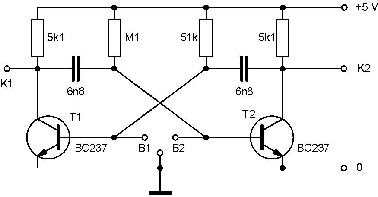
\includegraphics[scale=1.00]{scheme.png}
\caption{Schéma zapojení astabilního klopného obvodu s vyznačenými měřicími body}
\end{figure}
\begin{figure}[htp]
\centering
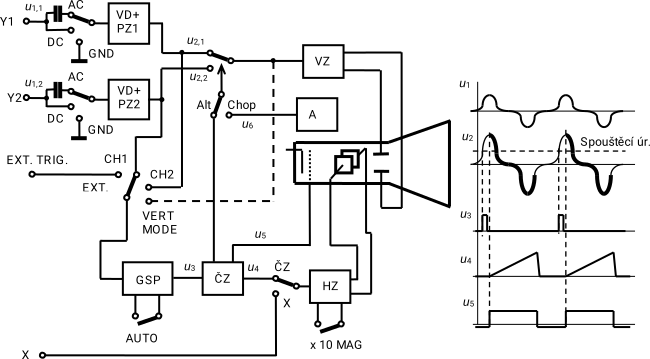
\includegraphics[scale=0.8]{block.png}
\caption{Osciloskop}
\end{figure}
\end{document}
